\documentclass[10pt]{article}
\usepackage{ucs}
\usepackage[a4paper, total={6in, 10in}]{geometry}
\usepackage[utf8x]{inputenc}
\usepackage{graphicx}
\title{Essential Skills: Assignment Computer architecture}
\date{2 October 2016}
\author{Ali Abdulmadzhidov}

\begin{document}
\renewcommand*\rmdefault{cmss}
\maketitle
\section{Digital circuit}
We add 1000 (right to left) from constant's. Output on leds is 1001.
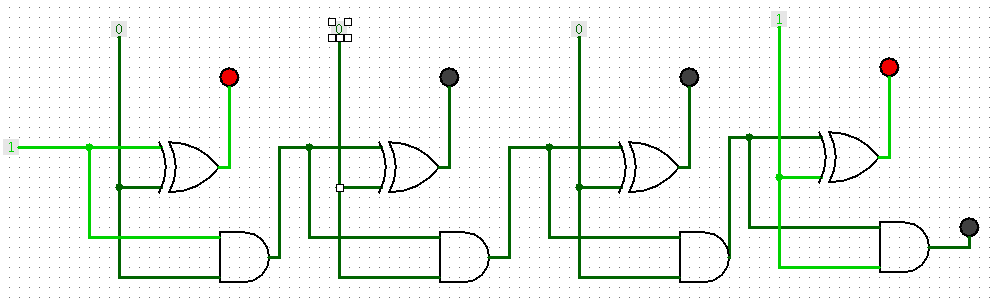
\includegraphics[width=\textwidth, scale=0.5]{circuit1} \\ \\
We add 1010 (right to left) from constant's. Output on leds is 1011
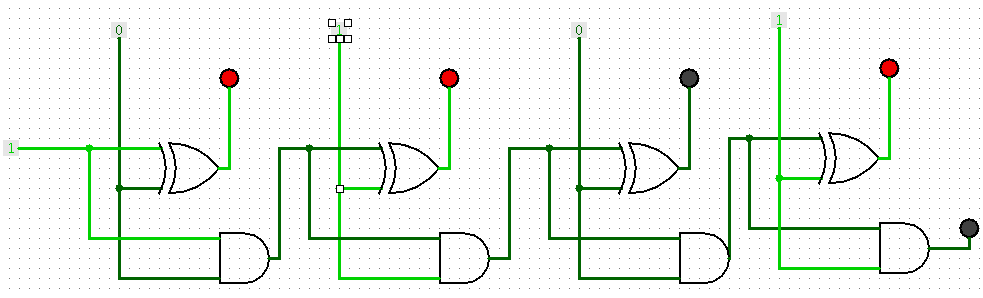
\includegraphics[width=\textwidth, scale=0.5]{circuit2} \\ \\

\section{title}


\end{document}